\documentclass[1p]{elsarticle_modified}
%\bibliographystyle{elsarticle-num}

%\usepackage[colorlinks]{hyperref}
%\usepackage{abbrmath_seonhwa} %\Abb, \Ascr, \Acal ,\Abf, \Afrak
\usepackage{amsfonts}
\usepackage{amssymb}
\usepackage{amsmath}
\usepackage{amsthm}
\usepackage{scalefnt}
\usepackage{amsbsy}
\usepackage{kotex}
\usepackage{caption}
\usepackage{subfig}
\usepackage{color}
\usepackage{graphicx}
\usepackage{xcolor} %% white, black, red, green, blue, cyan, magenta, yellow
\usepackage{float}
\usepackage{setspace}
\usepackage{hyperref}

\usepackage{tikz}
\usetikzlibrary{arrows}

\usepackage{multirow}
\usepackage{array} % fixed length table
\usepackage{hhline}

%%%%%%%%%%%%%%%%%%%%%
\makeatletter
\renewcommand*\env@matrix[1][\arraystretch]{%
	\edef\arraystretch{#1}%
	\hskip -\arraycolsep
	\let\@ifnextchar\new@ifnextchar
	\array{*\c@MaxMatrixCols c}}
\makeatother %https://tex.stackexchange.com/questions/14071/how-can-i-increase-the-line-spacing-in-a-matrix
%%%%%%%%%%%%%%%

\usepackage[normalem]{ulem}

\newcommand{\msout}[1]{\ifmmode\text{\sout{\ensuremath{#1}}}\else\sout{#1}\fi}
%SOURCE: \msout is \stkout macro in https://tex.stackexchange.com/questions/20609/strikeout-in-math-mode

\newcommand{\cancel}[1]{
	\ifmmode
	{\color{red}\msout{#1}}
	\else
	{\color{red}\sout{#1}}
	\fi
}

\newcommand{\add}[1]{
	{\color{blue}\uwave{#1}}
}

\newcommand{\replace}[2]{
	\ifmmode
	{\color{red}\msout{#1}}{\color{blue}\uwave{#2}}
	\else
	{\color{red}\sout{#1}}{\color{blue}\uwave{#2}}
	\fi
}

\newcommand{\Sol}{\mathcal{S}} %segment
\newcommand{\D}{D} %diagram
\newcommand{\A}{\mathcal{A}} %arc


%%%%%%%%%%%%%%%%%%%%%%%%%%%%%5 test

\def\sl{\operatorname{\textup{SL}}(2,\Cbb)}
\def\psl{\operatorname{\textup{PSL}}(2,\Cbb)}
\def\quan{\mkern 1mu \triangleright \mkern 1mu}

\theoremstyle{definition}
\newtheorem{thm}{Theorem}[section]
\newtheorem{prop}[thm]{Proposition}
\newtheorem{lem}[thm]{Lemma}
\newtheorem{ques}[thm]{Question}
\newtheorem{cor}[thm]{Corollary}
\newtheorem{defn}[thm]{Definition}
\newtheorem{exam}[thm]{Example}
\newtheorem{rmk}[thm]{Remark}
\newtheorem{alg}[thm]{Algorithm}

\newcommand{\I}{\sqrt{-1}}
\begin{document}

%\begin{frontmatter}
%
%\title{Boundary parabolic representations of knots up to 8 crossings}
%
%%% Group authors per affiliation:
%\author{Yunhi Cho} 
%\address{Department of Mathematics, University of Seoul, Seoul, Korea}
%\ead{yhcho@uos.ac.kr}
%
%
%\author{Seonhwa Kim} %\fnref{s_kim}}
%\address{Center for Geometry and Physics, Institute for Basic Science, Pohang, 37673, Korea}
%\ead{ryeona17@ibs.re.kr}
%
%\author{Hyuk Kim}
%\address{Department of Mathematical Sciences, Seoul National University, Seoul 08826, Korea}
%\ead{hyukkim@snu.ac.kr}
%
%\author{Seokbeom Yoon}
%\address{Department of Mathematical Sciences, Seoul National University, Seoul, 08826,  Korea}
%\ead{sbyoon15@snu.ac.kr}
%
%\begin{abstract}
%We find all boundary parabolic representation of knots up to 8 crossings.
%
%\end{abstract}
%\begin{keyword}
%    \MSC[2010] 57M25 
%\end{keyword}
%
%\end{frontmatter}

%\linenumbers
%\tableofcontents
%
\newcommand\colored[1]{\textcolor{white}{\rule[-0.35ex]{0.8em}{1.4ex}}\kern-0.8em\color{red} #1}%
%\newcommand\colored[1]{\textcolor{white}{ #1}\kern-2.17ex	\textcolor{white}{ #1}\kern-1.81ex	\textcolor{white}{ #1}\kern-2.15ex\color{red}#1	}

{\Large $\underline{12a_{0599}~(K12a_{0599})}$}

\setlength{\tabcolsep}{10pt}
\renewcommand{\arraystretch}{1.6}
\vspace{1cm}\begin{tabular}{m{100pt}>{\centering\arraybackslash}m{274pt}}
\multirow{5}{120pt}{
	\centering
	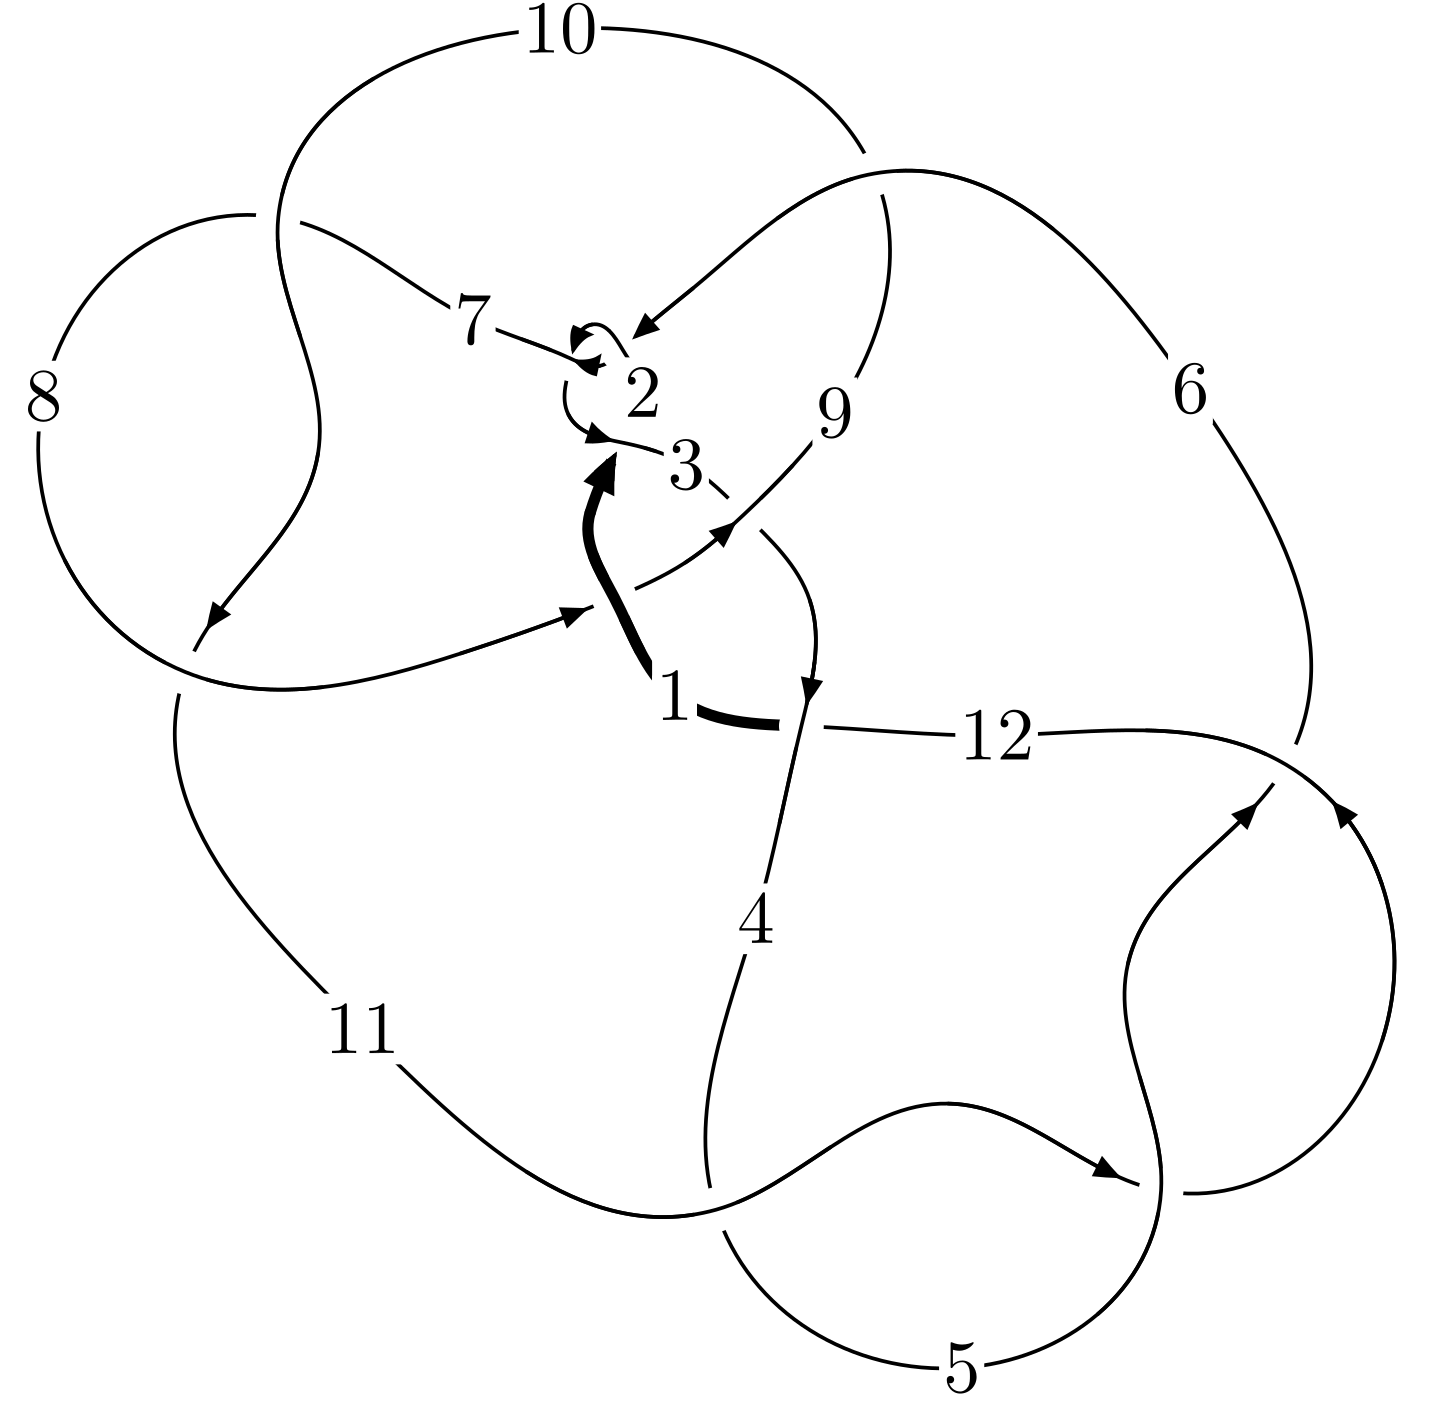
\includegraphics[width=112pt]{../../../GIT/diagram.site/Diagrams/png/1400_12a_0599.png}\\
\ \ \ A knot diagram\footnotemark}&
\allowdisplaybreaks
\textbf{Linearized knot diagam} \\
\cline{2-2}
 &
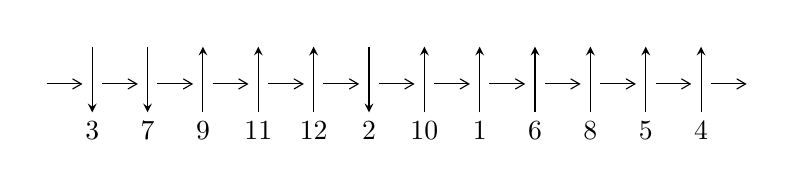
\begin{tikzpicture}[x=20pt, y=17pt]
	% nodes
	\node (C0) at (0, 0) {};
	\node (C1) at (1, 0) {};
	\node (C1U) at (1, +1) {};
	\node (C1D) at (1, -1) {3};

	\node (C2) at (2, 0) {};
	\node (C2U) at (2, +1) {};
	\node (C2D) at (2, -1) {7};

	\node (C3) at (3, 0) {};
	\node (C3U) at (3, +1) {};
	\node (C3D) at (3, -1) {9};

	\node (C4) at (4, 0) {};
	\node (C4U) at (4, +1) {};
	\node (C4D) at (4, -1) {11};

	\node (C5) at (5, 0) {};
	\node (C5U) at (5, +1) {};
	\node (C5D) at (5, -1) {12};

	\node (C6) at (6, 0) {};
	\node (C6U) at (6, +1) {};
	\node (C6D) at (6, -1) {2};

	\node (C7) at (7, 0) {};
	\node (C7U) at (7, +1) {};
	\node (C7D) at (7, -1) {10};

	\node (C8) at (8, 0) {};
	\node (C8U) at (8, +1) {};
	\node (C8D) at (8, -1) {1};

	\node (C9) at (9, 0) {};
	\node (C9U) at (9, +1) {};
	\node (C9D) at (9, -1) {6};

	\node (C10) at (10, 0) {};
	\node (C10U) at (10, +1) {};
	\node (C10D) at (10, -1) {8};

	\node (C11) at (11, 0) {};
	\node (C11U) at (11, +1) {};
	\node (C11D) at (11, -1) {5};

	\node (C12) at (12, 0) {};
	\node (C12U) at (12, +1) {};
	\node (C12D) at (12, -1) {4};
	\node (C13) at (13, 0) {};

	% arrows
	\draw[->,>={angle 60}]
	(C0) edge (C1) (C1) edge (C2) (C2) edge (C3) (C3) edge (C4) (C4) edge (C5) (C5) edge (C6) (C6) edge (C7) (C7) edge (C8) (C8) edge (C9) (C9) edge (C10) (C10) edge (C11) (C11) edge (C12) (C12) edge (C13) ;	\draw[->,>=stealth]
	(C1U) edge (C1D) (C2U) edge (C2D) (C3D) edge (C3U) (C4D) edge (C4U) (C5D) edge (C5U) (C6U) edge (C6D) (C7D) edge (C7U) (C8D) edge (C8U) (C9D) edge (C9U) (C10D) edge (C10U) (C11D) edge (C11U) (C12D) edge (C12U) ;
	\end{tikzpicture} \\
\hhline{~~} \\& 
\textbf{Solving Sequence} \\ \cline{2-2} 
 &
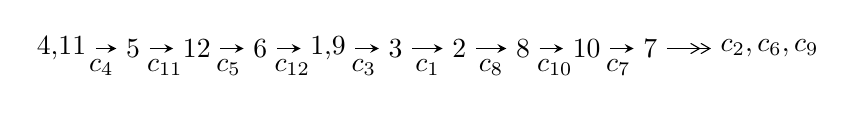
\begin{tikzpicture}[x=23pt, y=7pt]
	% node
	\node (A0) at (-1/8, 0) {4,11};
	\node (A1) at (1, 0) {5};
	\node (A2) at (2, 0) {12};
	\node (A3) at (3, 0) {6};
	\node (A4) at (65/16, 0) {1,9};
	\node (A5) at (41/8, 0) {3};
	\node (A6) at (49/8, 0) {2};
	\node (A7) at (57/8, 0) {8};
	\node (A8) at (65/8, 0) {10};
	\node (A9) at (73/8, 0) {7};
	\node (C1) at (1/2, -1) {$c_{4}$};
	\node (C2) at (3/2, -1) {$c_{11}$};
	\node (C3) at (5/2, -1) {$c_{5}$};
	\node (C4) at (7/2, -1) {$c_{12}$};
	\node (C5) at (37/8, -1) {$c_{3}$};
	\node (C6) at (45/8, -1) {$c_{1}$};
	\node (C7) at (53/8, -1) {$c_{8}$};
	\node (C8) at (61/8, -1) {$c_{10}$};
	\node (C9) at (69/8, -1) {$c_{7}$};
	\node (A10) at (11, 0) {$c_{2},c_{6},c_{9}$};

	% edge
	\draw[->,>=stealth]	
	(A0) edge (A1) (A1) edge (A2) (A2) edge (A3) (A3) edge (A4) (A4) edge (A5) (A5) edge (A6) (A6) edge (A7) (A7) edge (A8) (A8) edge (A9) ;
	\draw[->>,>={angle 60}]	
	(A9) edge (A10);
\end{tikzpicture} \\ 

\end{tabular} \\

\footnotetext{
The image of knot diagram is generated by the software ``\textbf{Draw programme}" developed by Andrew Bartholomew(\url{http://www.layer8.co.uk/maths/draw/index.htm\#Running-draw}), where we modified some parts for our purpose(\url{https://github.com/CATsTAILs/LinksPainter}).
}\phantom \\ \newline 
\centering \textbf{Ideals for irreducible components\footnotemark of $X_{\text{par}}$} 
 
\begin{align*}
I^u_{1}&=\langle 
-6.18140\times10^{106} u^{103}-1.68839\times10^{107} u^{102}+\cdots+8.40136\times10^{106} b-8.56625\times10^{106},\\
\phantom{I^u_{1}}&\phantom{= \langle  }1.80765\times10^{105} u^{103}+2.28944\times10^{105} u^{102}+\cdots+1.68027\times10^{106} a-7.57112\times10^{105},\;u^{104}+3 u^{103}+\cdots+2 u+1\rangle \\
\\
\end{align*}
\raggedright * 1 irreducible components of $\dim_{\mathbb{C}}=0$, with total 104 representations.\\
\footnotetext{All coefficients of polynomials are rational numbers. But the coefficients are sometimes approximated in decimal forms when there is not enough margin.}
\newpage
\renewcommand{\arraystretch}{1}
\centering \section*{I. $I^u_{1}= \langle -6.18\times10^{106} u^{103}-1.69\times10^{107} u^{102}+\cdots+8.40\times10^{106} b-8.57\times10^{106},\;1.81\times10^{105} u^{103}+2.29\times10^{105} u^{102}+\cdots+1.68\times10^{106} a-7.57\times10^{105},\;u^{104}+3 u^{103}+\cdots+2 u+1 \rangle$}
\flushleft \textbf{(i) Arc colorings}\\
\begin{tabular}{m{7pt} m{180pt} m{7pt} m{180pt} }
\flushright $a_{4}=$&$\begin{pmatrix}1\\0\end{pmatrix}$ \\
\flushright $a_{11}=$&$\begin{pmatrix}0\\u\end{pmatrix}$ \\
\flushright $a_{5}=$&$\begin{pmatrix}1\\- u^2\end{pmatrix}$ \\
\flushright $a_{12}=$&$\begin{pmatrix}u\\- u^3+u\end{pmatrix}$ \\
\flushright $a_{6}=$&$\begin{pmatrix}- u^2+1\\u^4-2 u^2\end{pmatrix}$ \\
\flushright $a_{1}=$&$\begin{pmatrix}- u^3+2 u\\- u^3+u\end{pmatrix}$ \\
\flushright $a_{9}=$&$\begin{pmatrix}-0.107581 u^{103}-0.136254 u^{102}+\cdots+5.30403 u+0.450589\\0.735762 u^{103}+2.00966 u^{102}+\cdots+2.25110 u+1.01963\end{pmatrix}$ \\
\flushright $a_{3}=$&$\begin{pmatrix}0.540322 u^{103}+0.963064 u^{102}+\cdots-4.53621 u-0.0896284\\-0.874844 u^{103}-2.38227 u^{102}+\cdots-2.60814 u-2.37733\end{pmatrix}$ \\
\flushright $a_{2}=$&$\begin{pmatrix}1.88927 u^{103}+5.89937 u^{102}+\cdots-0.482302 u+0.853416\\1.41968 u^{103}+4.11081 u^{102}+\cdots+1.60811 u+0.823482\end{pmatrix}$ \\
\flushright $a_{8}=$&$\begin{pmatrix}-0.340032 u^{103}-0.0211301 u^{102}+\cdots+4.20707 u-1.59516\\2.19574 u^{103}+4.81322 u^{102}+\cdots+3.24526 u+1.19118\end{pmatrix}$ \\
\flushright $a_{10}=$&$\begin{pmatrix}0.540859 u^{103}+2.31345 u^{102}+\cdots+5.26158 u-0.675638\\2.57621 u^{103}+6.00112 u^{102}+\cdots+4.56913 u+1.82368\end{pmatrix}$ \\
\flushright $a_{7}=$&$\begin{pmatrix}-2.37733 u^{103}-6.25714 u^{102}+\cdots-0.753556 u-2.14652\\-0.657904 u^{103}-2.25986 u^{102}+\cdots-1.17027 u-0.540322\end{pmatrix}$\\&\end{tabular}
\flushleft \textbf{(ii) Obstruction class $= -1$}\\~\\
\flushleft \textbf{(iii) Cusp Shapes $= 1.01554 u^{103}+4.88122 u^{102}+\cdots-15.4275 u+5.37327$}\\~\\
\newpage\renewcommand{\arraystretch}{1}
\flushleft \textbf{(iv) u-Polynomials at the component}\newline \\
\begin{tabular}{m{50pt}|m{274pt}}
Crossings & \hspace{64pt}u-Polynomials at each crossing \\
\hline $$\begin{aligned}c_{1}\end{aligned}$$&$\begin{aligned}
&u^{104}+39 u^{103}+\cdots+4 u+1
\end{aligned}$\\
\hline $$\begin{aligned}c_{2},c_{6}\end{aligned}$$&$\begin{aligned}
&u^{104}-3 u^{103}+\cdots-4 u+1
\end{aligned}$\\
\hline $$\begin{aligned}c_{3}\end{aligned}$$&$\begin{aligned}
&u^{104}- u^{103}+\cdots-22 u-1
\end{aligned}$\\
\hline $$\begin{aligned}c_{4},c_{5},c_{11}\end{aligned}$$&$\begin{aligned}
&u^{104}-3 u^{103}+\cdots-2 u+1
\end{aligned}$\\
\hline $$\begin{aligned}c_{7},c_{10}\end{aligned}$$&$\begin{aligned}
&u^{104}+u^{103}+\cdots+34 u-1
\end{aligned}$\\
\hline $$\begin{aligned}c_{8}\end{aligned}$$&$\begin{aligned}
&u^{104}+43 u^{103}+\cdots+121854 u+32269
\end{aligned}$\\
\hline $$\begin{aligned}c_{9}\end{aligned}$$&$\begin{aligned}
&u^{104}+5 u^{103}+\cdots-325970 u+195737
\end{aligned}$\\
\hline $$\begin{aligned}c_{12}\end{aligned}$$&$\begin{aligned}
&u^{104}+9 u^{103}+\cdots-5770 u-725
\end{aligned}$\\
\hline
\end{tabular}\\~\\
\newpage\renewcommand{\arraystretch}{1}
\flushleft \textbf{(v) Riley Polynomials at the component}\newline \\
\begin{tabular}{m{50pt}|m{274pt}}
Crossings & \hspace{64pt}Riley Polynomials at each crossing \\
\hline $$\begin{aligned}c_{1}\end{aligned}$$&$\begin{aligned}
&y^{104}+53 y^{103}+\cdots+28 y+1
\end{aligned}$\\
\hline $$\begin{aligned}c_{2},c_{6}\end{aligned}$$&$\begin{aligned}
&y^{104}-39 y^{103}+\cdots-4 y+1
\end{aligned}$\\
\hline $$\begin{aligned}c_{3}\end{aligned}$$&$\begin{aligned}
&y^{104}-3 y^{103}+\cdots-100 y+1
\end{aligned}$\\
\hline $$\begin{aligned}c_{4},c_{5},c_{11}\end{aligned}$$&$\begin{aligned}
&y^{104}-91 y^{103}+\cdots-4 y+1
\end{aligned}$\\
\hline $$\begin{aligned}c_{7},c_{10}\end{aligned}$$&$\begin{aligned}
&y^{104}-71 y^{103}+\cdots+844 y+1
\end{aligned}$\\
\hline $$\begin{aligned}c_{8}\end{aligned}$$&$\begin{aligned}
&y^{104}-575 y^{103}+\cdots-55858036808 y+1041288361
\end{aligned}$\\
\hline $$\begin{aligned}c_{9}\end{aligned}$$&$\begin{aligned}
&y^{104}+501 y^{103}+\cdots-1559554340176 y+38312973169
\end{aligned}$\\
\hline $$\begin{aligned}c_{12}\end{aligned}$$&$\begin{aligned}
&y^{104}+17 y^{103}+\cdots+2768600 y+525625
\end{aligned}$\\
\hline
\end{tabular}\\~\\
\newpage\flushleft \textbf{(vi) Complex Volumes and Cusp Shapes}
$$\begin{array}{c|c|c}  
\text{Solutions to }I^u_{1}& \I (\text{vol} + \sqrt{-1}CS) & \text{Cusp shape}\\
 \hline 
\begin{aligned}
u &= \phantom{-}0.989526 + 0.131041 I \\
a &= \phantom{-}0.883619 - 0.264649 I \\
b &= \phantom{-}0.740437 - 1.108110 I\end{aligned}
 & -0.14536 - 4.59513 I & \phantom{-0.000000 } 0 \\ \hline\begin{aligned}
u &= \phantom{-}0.989526 - 0.131041 I \\
a &= \phantom{-}0.883619 + 0.264649 I \\
b &= \phantom{-}0.740437 + 1.108110 I\end{aligned}
 & -0.14536 + 4.59513 I & \phantom{-0.000000 } 0 \\ \hline\begin{aligned}
u &= -0.846433 + 0.492394 I \\
a &= \phantom{-}0.824251 + 0.236983 I \\
b &= \phantom{-}0.921699 + 0.805391 I\end{aligned}
 & \phantom{-}5.21407 + 3.81898 I & \phantom{-0.000000 } 0 \\ \hline\begin{aligned}
u &= -0.846433 - 0.492394 I \\
a &= \phantom{-}0.824251 - 0.236983 I \\
b &= \phantom{-}0.921699 - 0.805391 I\end{aligned}
 & \phantom{-}5.21407 - 3.81898 I & \phantom{-0.000000 } 0 \\ \hline\begin{aligned}
u &= \phantom{-}0.846368 + 0.470568 I \\
a &= -0.896666 + 0.390579 I \\
b &= -0.970228 + 1.015240 I\end{aligned}
 & \phantom{-}3.57729 - 9.85375 I & \phantom{-0.000000 } 0 \\ \hline\begin{aligned}
u &= \phantom{-}0.846368 - 0.470568 I \\
a &= -0.896666 - 0.390579 I \\
b &= -0.970228 - 1.015240 I\end{aligned}
 & \phantom{-}3.57729 + 9.85375 I & \phantom{-0.000000 } 0 \\ \hline\begin{aligned}
u &= -0.345479 + 0.873329 I \\
a &= -0.329641 + 0.633256 I \\
b &= -0.515483 + 0.318246 I\end{aligned}
 & \phantom{-}2.33648 - 3.25638 I & \phantom{-0.000000 } 0 \\ \hline\begin{aligned}
u &= -0.345479 - 0.873329 I \\
a &= -0.329641 - 0.633256 I \\
b &= -0.515483 - 0.318246 I\end{aligned}
 & \phantom{-}2.33648 + 3.25638 I & \phantom{-0.000000 } 0 \\ \hline\begin{aligned}
u &= \phantom{-}0.168045 + 0.918321 I \\
a &= \phantom{-}0.681538 - 0.436064 I \\
b &= \phantom{-}0.399562 - 0.441746 I\end{aligned}
 & \phantom{-}0.23249 - 3.75946 I & \phantom{-0.000000 } 0 \\ \hline\begin{aligned}
u &= \phantom{-}0.168045 - 0.918321 I \\
a &= \phantom{-}0.681538 + 0.436064 I \\
b &= \phantom{-}0.399562 + 0.441746 I\end{aligned}
 & \phantom{-}0.23249 + 3.75946 I & \phantom{-0.000000 } 0\\
 \hline 
 \end{array}$$\newpage$$\begin{array}{c|c|c}  
\text{Solutions to }I^u_{1}& \I (\text{vol} + \sqrt{-1}CS) & \text{Cusp shape}\\
 \hline 
\begin{aligned}
u &= \phantom{-}1.038150 + 0.281331 I \\
a &= \phantom{-}0.574175 - 0.696383 I \\
b &= \phantom{-}0.171610 - 1.125820 I\end{aligned}
 & -3.13606 + 2.08755 I & \phantom{-0.000000 } 0 \\ \hline\begin{aligned}
u &= \phantom{-}1.038150 - 0.281331 I \\
a &= \phantom{-}0.574175 + 0.696383 I \\
b &= \phantom{-}0.171610 + 1.125820 I\end{aligned}
 & -3.13606 - 2.08755 I & \phantom{-0.000000 } 0 \\ \hline\begin{aligned}
u &= -1.088660 + 0.148356 I \\
a &= -0.569342 - 0.242387 I \\
b &= -0.601460 - 0.855575 I\end{aligned}
 & \phantom{-}1.47163 - 0.22582 I & \phantom{-0.000000 } 0 \\ \hline\begin{aligned}
u &= -1.088660 - 0.148356 I \\
a &= -0.569342 + 0.242387 I \\
b &= -0.601460 + 0.855575 I\end{aligned}
 & \phantom{-}1.47163 + 0.22582 I & \phantom{-0.000000 } 0 \\ \hline\begin{aligned}
u &= \phantom{-}1.021500 + 0.461685 I \\
a &= -0.132237 - 0.773987 I \\
b &= -0.637551 - 0.715827 I\end{aligned}
 & \phantom{-}2.90669 + 8.60744 I & \phantom{-0.000000 } 0 \\ \hline\begin{aligned}
u &= \phantom{-}1.021500 - 0.461685 I \\
a &= -0.132237 + 0.773987 I \\
b &= -0.637551 + 0.715827 I\end{aligned}
 & \phantom{-}2.90669 - 8.60744 I & \phantom{-0.000000 } 0 \\ \hline\begin{aligned}
u &= \phantom{-}0.714848 + 0.496575 I \\
a &= -0.391758 + 0.307832 I \\
b &= -0.268115 + 0.809910 I\end{aligned}
 & -2.18985 - 2.17775 I & \phantom{-0.000000 } 0 \\ \hline\begin{aligned}
u &= \phantom{-}0.714848 - 0.496575 I \\
a &= -0.391758 - 0.307832 I \\
b &= -0.268115 - 0.809910 I\end{aligned}
 & -2.18985 + 2.17775 I & \phantom{-0.000000 } 0 \\ \hline\begin{aligned}
u &= -0.277989 + 0.805746 I \\
a &= -0.43532 + 2.02951 I \\
b &= -1.04109 + 0.98300 I\end{aligned}
 & \phantom{-}3.40888 - 8.39494 I & \phantom{-0.000000 } 0 \\ \hline\begin{aligned}
u &= -0.277989 - 0.805746 I \\
a &= -0.43532 - 2.02951 I \\
b &= -1.04109 - 0.98300 I\end{aligned}
 & \phantom{-}3.40888 + 8.39494 I & \phantom{-0.000000 } 0\\
 \hline 
 \end{array}$$\newpage$$\begin{array}{c|c|c}  
\text{Solutions to }I^u_{1}& \I (\text{vol} + \sqrt{-1}CS) & \text{Cusp shape}\\
 \hline 
\begin{aligned}
u &= \phantom{-}0.271419 + 0.800534 I \\
a &= \phantom{-}0.32107 + 2.33269 I \\
b &= \phantom{-}1.07449 + 1.16223 I\end{aligned}
 & \phantom{-}1.7395 + 14.3608 I & \phantom{-}6.00000 - 9.55805 I \\ \hline\begin{aligned}
u &= \phantom{-}0.271419 - 0.800534 I \\
a &= \phantom{-}0.32107 - 2.33269 I \\
b &= \phantom{-}1.07449 - 1.16223 I\end{aligned}
 & \phantom{-}1.7395 - 14.3608 I & \phantom{-}6.00000 + 9.55805 I \\ \hline\begin{aligned}
u &= \phantom{-}0.301715 + 0.780914 I \\
a &= -0.25793 + 1.53795 I \\
b &= \phantom{-}0.565053 + 0.968257 I\end{aligned}
 & -3.64893 + 6.60879 I & \phantom{-0.000000 } 0. - 7.74517 I \\ \hline\begin{aligned}
u &= \phantom{-}0.301715 - 0.780914 I \\
a &= -0.25793 - 1.53795 I \\
b &= \phantom{-}0.565053 - 0.968257 I\end{aligned}
 & -3.64893 - 6.60879 I & \phantom{-0.000000 -}0. + 7.74517 I \\ \hline\begin{aligned}
u &= -1.048700 + 0.562138 I \\
a &= \phantom{-}0.176179 - 0.398546 I \\
b &= \phantom{-}0.471374 - 0.301344 I\end{aligned}
 & \phantom{-}4.38851 - 2.18462 I & \phantom{-0.000000 } 0 \\ \hline\begin{aligned}
u &= -1.048700 - 0.562138 I \\
a &= \phantom{-}0.176179 + 0.398546 I \\
b &= \phantom{-}0.471374 + 0.301344 I\end{aligned}
 & \phantom{-}4.38851 + 2.18462 I & \phantom{-0.000000 } 0 \\ \hline\begin{aligned}
u &= \phantom{-}0.162530 + 0.740437 I \\
a &= \phantom{-}0.17843 - 2.11043 I \\
b &= -0.437804 - 1.169340 I\end{aligned}
 & -5.77665 + 1.73251 I & -2.33025 - 1.80037 I \\ \hline\begin{aligned}
u &= \phantom{-}0.162530 - 0.740437 I \\
a &= \phantom{-}0.17843 + 2.11043 I \\
b &= -0.437804 + 1.169340 I\end{aligned}
 & -5.77665 - 1.73251 I & -2.33025 + 1.80037 I \\ \hline\begin{aligned}
u &= -1.248350 + 0.112459 I \\
a &= \phantom{-}0.226760 + 0.106758 I \\
b &= -0.791191 - 0.335299 I\end{aligned}
 & \phantom{-}2.16662 - 0.42827 I & \phantom{-0.000000 } 0 \\ \hline\begin{aligned}
u &= -1.248350 - 0.112459 I \\
a &= \phantom{-}0.226760 - 0.106758 I \\
b &= -0.791191 + 0.335299 I\end{aligned}
 & \phantom{-}2.16662 + 0.42827 I & \phantom{-0.000000 } 0\\
 \hline 
 \end{array}$$\newpage$$\begin{array}{c|c|c}  
\text{Solutions to }I^u_{1}& \I (\text{vol} + \sqrt{-1}CS) & \text{Cusp shape}\\
 \hline 
\begin{aligned}
u &= \phantom{-}0.201135 + 0.708814 I \\
a &= -0.65799 - 2.69199 I \\
b &= -1.17052 - 1.32325 I\end{aligned}
 & -2.39932 + 8.07353 I & \phantom{-}2.96084 - 8.86760 I \\ \hline\begin{aligned}
u &= \phantom{-}0.201135 - 0.708814 I \\
a &= -0.65799 + 2.69199 I \\
b &= -1.17052 + 1.32325 I\end{aligned}
 & -2.39932 - 8.07353 I & \phantom{-}2.96084 + 8.86760 I \\ \hline\begin{aligned}
u &= -0.186873 + 0.690936 I \\
a &= \phantom{-}0.77808 - 2.16675 I \\
b &= \phantom{-}1.12913 - 0.94113 I\end{aligned}
 & -1.00539 - 3.04538 I & \phantom{-}5.02927 + 4.37384 I \\ \hline\begin{aligned}
u &= -0.186873 - 0.690936 I \\
a &= \phantom{-}0.77808 + 2.16675 I \\
b &= \phantom{-}1.12913 + 0.94113 I\end{aligned}
 & -1.00539 + 3.04538 I & \phantom{-}5.02927 - 4.37384 I \\ \hline\begin{aligned}
u &= -1.280030 + 0.182164 I \\
a &= \phantom{-}2.30865 - 1.83870 I \\
b &= -0.533197 - 0.041483 I\end{aligned}
 & \phantom{-}4.29134 - 4.85987 I & \phantom{-0.000000 } 0 \\ \hline\begin{aligned}
u &= -1.280030 - 0.182164 I \\
a &= \phantom{-}2.30865 + 1.83870 I \\
b &= -0.533197 + 0.041483 I\end{aligned}
 & \phantom{-}4.29134 + 4.85987 I & \phantom{-0.000000 } 0 \\ \hline\begin{aligned}
u &= \phantom{-}1.308150 + 0.207596 I \\
a &= -12.4273 + 8.9998 I \\
b &= \phantom{-}0.0918274 + 0.0787198 I\end{aligned}
 & \phantom{-}4.66635 + 0.78468 I & \phantom{-0.000000 } 0 \\ \hline\begin{aligned}
u &= \phantom{-}1.308150 - 0.207596 I \\
a &= -12.4273 - 8.9998 I \\
b &= \phantom{-}0.0918274 - 0.0787198 I\end{aligned}
 & \phantom{-}4.66635 - 0.78468 I & \phantom{-0.000000 } 0 \\ \hline\begin{aligned}
u &= \phantom{-}1.320460 + 0.153660 I \\
a &= -1.46352 + 0.79473 I \\
b &= \phantom{-}0.811793 + 0.351138 I\end{aligned}
 & \phantom{-}5.21559 + 1.16431 I & \phantom{-0.000000 } 0 \\ \hline\begin{aligned}
u &= \phantom{-}1.320460 - 0.153660 I \\
a &= -1.46352 - 0.79473 I \\
b &= \phantom{-}0.811793 - 0.351138 I\end{aligned}
 & \phantom{-}5.21559 - 1.16431 I & \phantom{-0.000000 } 0\\
 \hline 
 \end{array}$$\newpage$$\begin{array}{c|c|c}  
\text{Solutions to }I^u_{1}& \I (\text{vol} + \sqrt{-1}CS) & \text{Cusp shape}\\
 \hline 
\begin{aligned}
u &= -1.310210 + 0.236069 I \\
a &= -0.157080 - 1.091820 I \\
b &= \phantom{-}0.160988 - 0.095874 I\end{aligned}
 & \phantom{-}3.04010 - 0.83758 I & \phantom{-0.000000 } 0 \\ \hline\begin{aligned}
u &= -1.310210 - 0.236069 I \\
a &= -0.157080 + 1.091820 I \\
b &= \phantom{-}0.160988 + 0.095874 I\end{aligned}
 & \phantom{-}3.04010 + 0.83758 I & \phantom{-0.000000 } 0 \\ \hline\begin{aligned}
u &= -1.343800 + 0.078810 I \\
a &= \phantom{-}0.382497 + 1.052170 I \\
b &= -1.57134 - 0.37622 I\end{aligned}
 & \phantom{-}5.39810 + 4.39371 I & \phantom{-0.000000 } 0 \\ \hline\begin{aligned}
u &= -1.343800 - 0.078810 I \\
a &= \phantom{-}0.382497 - 1.052170 I \\
b &= -1.57134 + 0.37622 I\end{aligned}
 & \phantom{-}5.39810 - 4.39371 I & \phantom{-0.000000 } 0 \\ \hline\begin{aligned}
u &= \phantom{-}1.342890 + 0.103976 I \\
a &= -0.658717 + 1.060560 I \\
b &= \phantom{-}1.54649 + 0.00805 I\end{aligned}
 & \phantom{-}6.33561 + 0.56533 I & \phantom{-0.000000 } 0 \\ \hline\begin{aligned}
u &= \phantom{-}1.342890 - 0.103976 I \\
a &= -0.658717 - 1.060560 I \\
b &= \phantom{-}1.54649 - 0.00805 I\end{aligned}
 & \phantom{-}6.33561 - 0.56533 I & \phantom{-0.000000 } 0 \\ \hline\begin{aligned}
u &= \phantom{-}1.338520 + 0.257583 I \\
a &= \phantom{-}0.74243 - 1.24808 I \\
b &= -0.711072 - 0.202051 I\end{aligned}
 & \phantom{-}3.75246 + 5.21120 I & \phantom{-0.000000 } 0 \\ \hline\begin{aligned}
u &= \phantom{-}1.338520 - 0.257583 I \\
a &= \phantom{-}0.74243 + 1.24808 I \\
b &= -0.711072 + 0.202051 I\end{aligned}
 & \phantom{-}3.75246 - 5.21120 I & \phantom{-0.000000 } 0 \\ \hline\begin{aligned}
u &= \phantom{-}1.345000 + 0.244038 I \\
a &= \phantom{-}1.001560 - 0.942439 I \\
b &= -0.814953 + 0.094462 I\end{aligned}
 & \phantom{-}3.81873 + 5.22294 I & \phantom{-0.000000 } 0 \\ \hline\begin{aligned}
u &= \phantom{-}1.345000 - 0.244038 I \\
a &= \phantom{-}1.001560 + 0.942439 I \\
b &= -0.814953 - 0.094462 I\end{aligned}
 & \phantom{-}3.81873 - 5.22294 I & \phantom{-0.000000 } 0\\
 \hline 
 \end{array}$$\newpage$$\begin{array}{c|c|c}  
\text{Solutions to }I^u_{1}& \I (\text{vol} + \sqrt{-1}CS) & \text{Cusp shape}\\
 \hline 
\begin{aligned}
u &= -1.353180 + 0.207483 I \\
a &= \phantom{-}0.161585 + 0.980965 I \\
b &= \phantom{-}0.347548 + 0.906497 I\end{aligned}
 & \phantom{-}6.06988 - 3.47205 I & \phantom{-0.000000 } 0 \\ \hline\begin{aligned}
u &= -1.353180 - 0.207483 I \\
a &= \phantom{-}0.161585 - 0.980965 I \\
b &= \phantom{-}0.347548 - 0.906497 I\end{aligned}
 & \phantom{-}6.06988 + 3.47205 I & \phantom{-0.000000 } 0 \\ \hline\begin{aligned}
u &= -0.103587 + 0.622209 I \\
a &= \phantom{-}0.287222 - 1.328960 I \\
b &= \phantom{-}0.475281 - 0.083983 I\end{aligned}
 & -0.80872 - 1.97143 I & \phantom{-}3.33449 + 4.65511 I \\ \hline\begin{aligned}
u &= -0.103587 - 0.622209 I \\
a &= \phantom{-}0.287222 + 1.328960 I \\
b &= \phantom{-}0.475281 + 0.083983 I\end{aligned}
 & -0.80872 + 1.97143 I & \phantom{-}3.33449 - 4.65511 I \\ \hline\begin{aligned}
u &= -0.142575 + 0.614426 I \\
a &= \phantom{-}0.280636 - 0.888346 I \\
b &= \phantom{-}0.811142 - 0.030751 I\end{aligned}
 & -0.87795 - 2.08035 I & \phantom{-}2.20405 + 5.01346 I \\ \hline\begin{aligned}
u &= -0.142575 - 0.614426 I \\
a &= \phantom{-}0.280636 + 0.888346 I \\
b &= \phantom{-}0.811142 + 0.030751 I\end{aligned}
 & -0.87795 + 2.08035 I & \phantom{-}2.20405 - 5.01346 I \\ \hline\begin{aligned}
u &= \phantom{-}0.621086 + 0.084207 I \\
a &= \phantom{-}0.373074 - 0.207627 I \\
b &= \phantom{-}0.760421 + 0.785124 I\end{aligned}
 & -0.13085 + 4.71370 I & \phantom{-}6.12729 - 5.66701 I \\ \hline\begin{aligned}
u &= \phantom{-}0.621086 - 0.084207 I \\
a &= \phantom{-}0.373074 + 0.207627 I \\
b &= \phantom{-}0.760421 - 0.785124 I\end{aligned}
 & -0.13085 - 4.71370 I & \phantom{-}6.12729 + 5.66701 I \\ \hline\begin{aligned}
u &= -0.241643 + 0.573906 I \\
a &= \phantom{-}2.38786 + 0.68773 I \\
b &= \phantom{-}1.52226 + 0.87466 I\end{aligned}
 & \phantom{-}2.66071 - 5.66668 I & \phantom{-}8.90037 + 9.71585 I \\ \hline\begin{aligned}
u &= -0.241643 - 0.573906 I \\
a &= \phantom{-}2.38786 - 0.68773 I \\
b &= \phantom{-}1.52226 - 0.87466 I\end{aligned}
 & \phantom{-}2.66071 + 5.66668 I & \phantom{-}8.90037 - 9.71585 I\\
 \hline 
 \end{array}$$\newpage$$\begin{array}{c|c|c}  
\text{Solutions to }I^u_{1}& \I (\text{vol} + \sqrt{-1}CS) & \text{Cusp shape}\\
 \hline 
\begin{aligned}
u &= \phantom{-}1.376580 + 0.166688 I \\
a &= -1.39265 + 1.24070 I \\
b &= \phantom{-}0.99625 + 1.78378 I\end{aligned}
 & \phantom{-}8.70992 - 0.92166 I & \phantom{-0.000000 } 0 \\ \hline\begin{aligned}
u &= \phantom{-}1.376580 - 0.166688 I \\
a &= -1.39265 - 1.24070 I \\
b &= \phantom{-}0.99625 - 1.78378 I\end{aligned}
 & \phantom{-}8.70992 + 0.92166 I & \phantom{-0.000000 } 0 \\ \hline\begin{aligned}
u &= -1.378030 + 0.177745 I \\
a &= \phantom{-}1.41515 + 1.05782 I \\
b &= -0.55253 + 1.95449 I\end{aligned}
 & \phantom{-}8.91266 - 4.20677 I & \phantom{-0.000000 } 0 \\ \hline\begin{aligned}
u &= -1.378030 - 0.177745 I \\
a &= \phantom{-}1.41515 - 1.05782 I \\
b &= -0.55253 - 1.95449 I\end{aligned}
 & \phantom{-}8.91266 + 4.20677 I & \phantom{-0.000000 } 0 \\ \hline\begin{aligned}
u &= -1.357880 + 0.299840 I \\
a &= -1.12463 - 1.04934 I \\
b &= \phantom{-}0.614318 - 1.177360 I\end{aligned}
 & -0.97490 - 5.49155 I & \phantom{-0.000000 } 0 \\ \hline\begin{aligned}
u &= -1.357880 - 0.299840 I \\
a &= -1.12463 + 1.04934 I \\
b &= \phantom{-}0.614318 + 1.177360 I\end{aligned}
 & -0.97490 + 5.49155 I & \phantom{-0.000000 } 0 \\ \hline\begin{aligned}
u &= \phantom{-}0.264003 + 0.545428 I \\
a &= -0.773141 - 0.191095 I \\
b &= -0.147180 + 0.538599 I\end{aligned}
 & -1.60451 - 1.80811 I & \phantom{-}0.324463 - 0.433644 I \\ \hline\begin{aligned}
u &= \phantom{-}0.264003 - 0.545428 I \\
a &= -0.773141 + 0.191095 I \\
b &= -0.147180 - 0.538599 I\end{aligned}
 & -1.60451 + 1.80811 I & \phantom{-}0.324463 + 0.433644 I \\ \hline\begin{aligned}
u &= \phantom{-}1.370800 + 0.278221 I \\
a &= \phantom{-}0.91185 - 1.51022 I \\
b &= -1.39185 - 1.01737 I\end{aligned}
 & \phantom{-}3.93475 + 6.56935 I & \phantom{-0.000000 } 0 \\ \hline\begin{aligned}
u &= \phantom{-}1.370800 - 0.278221 I \\
a &= \phantom{-}0.91185 + 1.51022 I \\
b &= -1.39185 + 1.01737 I\end{aligned}
 & \phantom{-}3.93475 - 6.56935 I & \phantom{-0.000000 } 0\\
 \hline 
 \end{array}$$\newpage$$\begin{array}{c|c|c}  
\text{Solutions to }I^u_{1}& \I (\text{vol} + \sqrt{-1}CS) & \text{Cusp shape}\\
 \hline 
\begin{aligned}
u &= -1.381400 + 0.222297 I \\
a &= \phantom{-}0.824612 - 0.474541 I \\
b &= \phantom{-}1.46910 + 1.43358 I\end{aligned}
 & \phantom{-}8.29547 - 3.50526 I & \phantom{-0.000000 } 0 \\ \hline\begin{aligned}
u &= -1.381400 - 0.222297 I \\
a &= \phantom{-}0.824612 + 0.474541 I \\
b &= \phantom{-}1.46910 - 1.43358 I\end{aligned}
 & \phantom{-}8.29547 + 3.50526 I & \phantom{-0.000000 } 0 \\ \hline\begin{aligned}
u &= \phantom{-}1.383110 + 0.231040 I \\
a &= -0.666482 - 0.888282 I \\
b &= -1.83700 + 1.13231 I\end{aligned}
 & \phantom{-}7.81652 + 8.64316 I & \phantom{-0.000000 } 0 \\ \hline\begin{aligned}
u &= \phantom{-}1.383110 - 0.231040 I \\
a &= -0.666482 + 0.888282 I \\
b &= -1.83700 - 1.13231 I\end{aligned}
 & \phantom{-}7.81652 - 8.64316 I & \phantom{-0.000000 } 0 \\ \hline\begin{aligned}
u &= -0.031347 + 0.595167 I \\
a &= -6.20853 - 6.78983 I \\
b &= \phantom{-}0.207524 - 0.127759 I\end{aligned}
 & \phantom{-}0.49697 + 2.09340 I & \phantom{-}27.5744 + 57.2719 I \\ \hline\begin{aligned}
u &= -0.031347 - 0.595167 I \\
a &= -6.20853 + 6.78983 I \\
b &= \phantom{-}0.207524 + 0.127759 I\end{aligned}
 & \phantom{-}0.49697 - 2.09340 I & \phantom{-}27.5744 - 57.2719 I \\ \hline\begin{aligned}
u &= \phantom{-}0.242443 + 0.543233 I \\
a &= -2.10102 + 1.43682 I \\
b &= -1.17748 + 1.11016 I\end{aligned}
 & \phantom{-}3.14800 + 0.65168 I & \phantom{-}10.52306 - 3.36761 I \\ \hline\begin{aligned}
u &= \phantom{-}0.242443 - 0.543233 I \\
a &= -2.10102 - 1.43682 I \\
b &= -1.17748 - 1.11016 I\end{aligned}
 & \phantom{-}3.14800 - 0.65168 I & \phantom{-}10.52306 + 3.36761 I \\ \hline\begin{aligned}
u &= -1.376820 + 0.285343 I \\
a &= -1.15345 - 1.60765 I \\
b &= \phantom{-}1.39674 - 1.41467 I\end{aligned}
 & \phantom{-}2.60570 - 11.68300 I & \phantom{-0.000000 } 0 \\ \hline\begin{aligned}
u &= -1.376820 - 0.285343 I \\
a &= -1.15345 + 1.60765 I \\
b &= \phantom{-}1.39674 + 1.41467 I\end{aligned}
 & \phantom{-}2.60570 + 11.68300 I & \phantom{-0.000000 } 0\\
 \hline 
 \end{array}$$\newpage$$\begin{array}{c|c|c}  
\text{Solutions to }I^u_{1}& \I (\text{vol} + \sqrt{-1}CS) & \text{Cusp shape}\\
 \hline 
\begin{aligned}
u &= -1.41904 + 0.32371 I \\
a &= \phantom{-}1.07007 + 1.52516 I \\
b &= -1.17872 + 1.21776 I\end{aligned}
 & \phantom{-}7.1225 - 18.4287 I & \phantom{-0.000000 } 0 \\ \hline\begin{aligned}
u &= -1.41904 - 0.32371 I \\
a &= \phantom{-}1.07007 - 1.52516 I \\
b &= -1.17872 - 1.21776 I\end{aligned}
 & \phantom{-}7.1225 + 18.4287 I & \phantom{-0.000000 } 0 \\ \hline\begin{aligned}
u &= \phantom{-}1.42240 + 0.32497 I \\
a &= -0.87371 + 1.42713 I \\
b &= \phantom{-}1.16421 + 1.04993 I\end{aligned}
 & \phantom{-}8.8252 + 12.4850 I & \phantom{-0.000000 } 0 \\ \hline\begin{aligned}
u &= \phantom{-}1.42240 - 0.32497 I \\
a &= -0.87371 - 1.42713 I \\
b &= \phantom{-}1.16421 - 1.04993 I\end{aligned}
 & \phantom{-}8.8252 - 12.4850 I & \phantom{-0.000000 } 0 \\ \hline\begin{aligned}
u &= -1.42942 + 0.31413 I \\
a &= \phantom{-}0.967730 + 0.879064 I \\
b &= -0.751390 + 0.981643 I\end{aligned}
 & \phantom{-}1.87186 - 10.58530 I & \phantom{-0.000000 } 0 \\ \hline\begin{aligned}
u &= -1.42942 - 0.31413 I \\
a &= \phantom{-}0.967730 - 0.879064 I \\
b &= -0.751390 - 0.981643 I\end{aligned}
 & \phantom{-}1.87186 + 10.58530 I & \phantom{-0.000000 } 0 \\ \hline\begin{aligned}
u &= \phantom{-}1.44617 + 0.33353 I \\
a &= -0.315245 + 0.785569 I \\
b &= \phantom{-}0.809528 + 0.474654 I\end{aligned}
 & \phantom{-}8.03571 + 7.55819 I & \phantom{-0.000000 } 0 \\ \hline\begin{aligned}
u &= \phantom{-}1.44617 - 0.33353 I \\
a &= -0.315245 - 0.785569 I \\
b &= \phantom{-}0.809528 - 0.474654 I\end{aligned}
 & \phantom{-}8.03571 - 7.55819 I & \phantom{-0.000000 } 0 \\ \hline\begin{aligned}
u &= \phantom{-}0.129827 + 0.487589 I \\
a &= \phantom{-}0.25714 + 2.36854 I \\
b &= -0.368575 + 0.570292 I\end{aligned}
 & \phantom{-}1.33150 + 0.83954 I & \phantom{-}4.54914 + 0.82518 I \\ \hline\begin{aligned}
u &= \phantom{-}0.129827 - 0.487589 I \\
a &= \phantom{-}0.25714 - 2.36854 I \\
b &= -0.368575 - 0.570292 I\end{aligned}
 & \phantom{-}1.33150 - 0.83954 I & \phantom{-}4.54914 - 0.82518 I\\
 \hline 
 \end{array}$$\newpage$$\begin{array}{c|c|c}  
\text{Solutions to }I^u_{1}& \I (\text{vol} + \sqrt{-1}CS) & \text{Cusp shape}\\
 \hline 
\begin{aligned}
u &= -1.50071 + 0.02299 I \\
a &= -0.394330 - 0.207023 I \\
b &= \phantom{-}1.157920 + 0.717227 I\end{aligned}
 & \phantom{-}11.3902 + 8.8099 I & \phantom{-0.000000 } 0 \\ \hline\begin{aligned}
u &= -1.50071 - 0.02299 I \\
a &= -0.394330 + 0.207023 I \\
b &= \phantom{-}1.157920 - 0.717227 I\end{aligned}
 & \phantom{-}11.3902 - 8.8099 I & \phantom{-0.000000 } 0 \\ \hline\begin{aligned}
u &= \phantom{-}1.50978 + 0.01787 I \\
a &= \phantom{-}0.369926 - 0.133517 I \\
b &= -1.156850 + 0.453893 I\end{aligned}
 & \phantom{-}13.17090 - 2.70458 I & \phantom{-0.000000 } 0 \\ \hline\begin{aligned}
u &= \phantom{-}1.50978 - 0.01787 I \\
a &= \phantom{-}0.369926 + 0.133517 I \\
b &= -1.156850 - 0.453893 I\end{aligned}
 & \phantom{-}13.17090 + 2.70458 I & \phantom{-0.000000 } 0 \\ \hline\begin{aligned}
u &= \phantom{-}0.302753 + 0.373014 I \\
a &= -1.08166 + 3.47219 I \\
b &= \phantom{-}0.443702 + 1.333090 I\end{aligned}
 & \phantom{-}3.69173 + 2.02129 I & \phantom{-}11.76908 - 5.97446 I \\ \hline\begin{aligned}
u &= \phantom{-}0.302753 - 0.373014 I \\
a &= -1.08166 - 3.47219 I \\
b &= \phantom{-}0.443702 - 1.333090 I\end{aligned}
 & \phantom{-}3.69173 - 2.02129 I & \phantom{-}11.76908 + 5.97446 I \\ \hline\begin{aligned}
u &= -0.337844 + 0.323246 I \\
a &= \phantom{-}0.77129 + 3.39601 I \\
b &= -0.824085 + 1.122500 I\end{aligned}
 & \phantom{-}3.45433 + 2.90974 I & \phantom{-}11.59556 - 0.92056 I \\ \hline\begin{aligned}
u &= -0.337844 - 0.323246 I \\
a &= \phantom{-}0.77129 - 3.39601 I \\
b &= -0.824085 - 1.122500 I\end{aligned}
 & \phantom{-}3.45433 - 2.90974 I & \phantom{-}11.59556 + 0.92056 I \\ \hline\begin{aligned}
u &= -0.460462 + 0.007635 I \\
a &= \phantom{-}0.126962 + 0.726061 I \\
b &= -0.808530 - 0.289273 I\end{aligned}
 & \phantom{-}1.167780 + 0.139175 I & \phantom{-}10.38139 - 0.59279 I \\ \hline\begin{aligned}
u &= -0.460462 - 0.007635 I \\
a &= \phantom{-}0.126962 - 0.726061 I \\
b &= -0.808530 + 0.289273 I\end{aligned}
 & \phantom{-}1.167780 - 0.139175 I & \phantom{-}10.38139 + 0.59279 I\\
 \hline 
 \end{array}$$\newpage$$\begin{array}{c|c|c}  
\text{Solutions to }I^u_{1}& \I (\text{vol} + \sqrt{-1}CS) & \text{Cusp shape}\\
 \hline 
\begin{aligned}
u &= -1.49255 + 0.37784 I \\
a &= \phantom{-}0.002911 + 0.308059 I \\
b &= -0.431301 + 0.112831 I\end{aligned}
 & \phantom{-}5.52489 - 1.27377 I & \phantom{-0.000000 } 0 \\ \hline\begin{aligned}
u &= -1.49255 - 0.37784 I \\
a &= \phantom{-}0.002911 - 0.308059 I \\
b &= -0.431301 - 0.112831 I\end{aligned}
 & \phantom{-}5.52489 + 1.27377 I & \phantom{-0.000000 } 0 \\ \hline\begin{aligned}
u &= -1.59052\phantom{ +0.000000I} \\
a &= -0.115804\phantom{ +0.000000I} \\
b &= \phantom{-}0.474770\phantom{ +0.000000I}\end{aligned}
 & \phantom{-}5.77568\phantom{ +0.000000I} & \phantom{-0.000000 } 0 \\ \hline\begin{aligned}
u &= -0.321853\phantom{ +0.000000I} \\
a &= \phantom{-}1.46602\phantom{ +0.000000I} \\
b &= -0.616577\phantom{ +0.000000I}\end{aligned}
 & \phantom{-}0.922749\phantom{ +0.000000I} & \phantom{-}11.9180\phantom{ +0.000000I}\\
 \hline 
 \end{array}$$\newpage
\newpage\renewcommand{\arraystretch}{1}
\centering \section*{ II. u-Polynomials}
\begin{tabular}{m{50pt}|m{274pt}}
Crossings & \hspace{64pt}u-Polynomials at each crossing \\
\hline $$\begin{aligned}c_{1}\end{aligned}$$&$\begin{aligned}
&u^{104}+39 u^{103}+\cdots+4 u+1
\end{aligned}$\\
\hline $$\begin{aligned}c_{2},c_{6}\end{aligned}$$&$\begin{aligned}
&u^{104}-3 u^{103}+\cdots-4 u+1
\end{aligned}$\\
\hline $$\begin{aligned}c_{3}\end{aligned}$$&$\begin{aligned}
&u^{104}- u^{103}+\cdots-22 u-1
\end{aligned}$\\
\hline $$\begin{aligned}c_{4},c_{5},c_{11}\end{aligned}$$&$\begin{aligned}
&u^{104}-3 u^{103}+\cdots-2 u+1
\end{aligned}$\\
\hline $$\begin{aligned}c_{7},c_{10}\end{aligned}$$&$\begin{aligned}
&u^{104}+u^{103}+\cdots+34 u-1
\end{aligned}$\\
\hline $$\begin{aligned}c_{8}\end{aligned}$$&$\begin{aligned}
&u^{104}+43 u^{103}+\cdots+121854 u+32269
\end{aligned}$\\
\hline $$\begin{aligned}c_{9}\end{aligned}$$&$\begin{aligned}
&u^{104}+5 u^{103}+\cdots-325970 u+195737
\end{aligned}$\\
\hline $$\begin{aligned}c_{12}\end{aligned}$$&$\begin{aligned}
&u^{104}+9 u^{103}+\cdots-5770 u-725
\end{aligned}$\\
\hline
\end{tabular}\newpage\renewcommand{\arraystretch}{1}
\centering \section*{ III. Riley Polynomials}
\begin{tabular}{m{50pt}|m{274pt}}
Crossings & \hspace{64pt}Riley Polynomials at each crossing \\
\hline $$\begin{aligned}c_{1}\end{aligned}$$&$\begin{aligned}
&y^{104}+53 y^{103}+\cdots+28 y+1
\end{aligned}$\\
\hline $$\begin{aligned}c_{2},c_{6}\end{aligned}$$&$\begin{aligned}
&y^{104}-39 y^{103}+\cdots-4 y+1
\end{aligned}$\\
\hline $$\begin{aligned}c_{3}\end{aligned}$$&$\begin{aligned}
&y^{104}-3 y^{103}+\cdots-100 y+1
\end{aligned}$\\
\hline $$\begin{aligned}c_{4},c_{5},c_{11}\end{aligned}$$&$\begin{aligned}
&y^{104}-91 y^{103}+\cdots-4 y+1
\end{aligned}$\\
\hline $$\begin{aligned}c_{7},c_{10}\end{aligned}$$&$\begin{aligned}
&y^{104}-71 y^{103}+\cdots+844 y+1
\end{aligned}$\\
\hline $$\begin{aligned}c_{8}\end{aligned}$$&$\begin{aligned}
&y^{104}-575 y^{103}+\cdots-55858036808 y+1041288361
\end{aligned}$\\
\hline $$\begin{aligned}c_{9}\end{aligned}$$&$\begin{aligned}
&y^{104}+501 y^{103}+\cdots-1559554340176 y+38312973169
\end{aligned}$\\
\hline $$\begin{aligned}c_{12}\end{aligned}$$&$\begin{aligned}
&y^{104}+17 y^{103}+\cdots+2768600 y+525625
\end{aligned}$\\
\hline
\end{tabular}
\vskip 2pc
\end{document}